\documentclass[11pt]{article}
\usepackage[left=1in,right=1in,top=1in,bottom=1in]{geometry}
\geometry{a4paper}

\usepackage{babel}
\usepackage[table]{xcolor}
\usepackage[utf8]{inputenc}
%\usepackage[T1]{fontenc}
\usepackage{amsfonts}
\usepackage{ragged2e}
\usepackage{amsmath}
\usepackage{amssymb}
\usepackage{graphicx}
\usepackage{wrapfig}
\usepackage{physics}
\usepackage{hyperref}
\usepackage{ragged2e}
\usepackage{float}
\usepackage{rotating}
\usepackage{ulem}
\usepackage{authblk}

\usepackage[
backend=bibtex,
%style=ieee
maxbibnames=3,
%backend=bibtex,
style=ieee
]{biblatex}
\addbibresource{./ref/golec.bib}
\addbibresource{./ref/gbw1998.bib}
\addbibresource{./ref/bgk2002.bib}
\addbibresource{./ref/impact.bib}
\addbibresource{./ref/cambqcd.bib}
\addbibresource{./ref/gbs2018.bib}
\addbibresource{./ref/gbs2006.bib}
\addbibresource{./ref/xiao2017.bib}
\addbibresource{./ref/minuit.bib}
\addbibresource{./ref/hera.bib}
\addbibresource{./ref/jk2006.bib}
\addbibresource{./ref/FL.bib}
\addbibresource{./ref/stasto2018.bib}
\addbibresource{./ref/stebel2020.bib}
\addbibresource{./ref/ellis1996.bib}
\addbibresource{./ref/bronstein.bib}
\addbibresource{./ref/mueller2016.bib}
\addbibresource{./ref/css1985.bib}
\addbibresource{./ref/prokudin2015.bib}
\addbibresource{./ref/collins2016.bib}

\newcommand{\pairdot}[2]{ \mathbf{#1}\cdot\mathbf{#2}  }
\begin{document}
\author{Krzystof Kutak, Sebastian Sapeta, Tomoki Goda
}	 
\title{ Effects of Sudakov form factor in\\ the
Golec-Biernat W\"usthoff saturation model}
\date{\today}
%\frontmatter
\maketitle
%\tableofcontents


\pagenumbering{arabic}
\numberwithin{equation}{section}
\numberwithin{table}{section}

\begin{abstract}

\end{abstract}

\section{Introduction}


In the dipole picture of deep inelastic scattering (DIS), a photon with virtuality $Q^2$ fluctuates into a pair of quark and antiquark, with momentum fractions $z$ and $(1-z)$ respectively, long before the interaction with the nucleon. Then the cross-section of inclusive DIS involves with the photon with polarization $P$, is factorized into the form \cite{gbw1998}%{\color{blue} correction. it is written `cf.' since this is not the original paper to have derived this factorization.  }
\begin{equation}
\sigma^{\gamma^* p}_{P}(x,Q^2)=\int d^2 \mathbf{r} \int^1_0 dz |\Psi_{P}(z,\mathbf{r})|^2 \sigma_{\mathrm{dp}}(x,r),
\label{eq:factorization}
\end{equation}
where the photon wave function, $\Psi_P(z, \mathbf{r}) $, describes the decay of a virtual photon into a quark-antiquark pair separated by the dipole size $r$, and the dipole cross-section, $\sigma_{\mathrm{dp}}(x,r)$, describes the interaction of the quark/antiquark with the target proton. 

The photon wave functions read  \cite{gbw1998}%{\color{blue} the same reason as above.}
\begin{align}
|\Psi_{T}(z,r,Q)|^2 & =\alpha_{em}\frac{3}{2\pi^2}\sum_{f=\{u,d,c,\dots\}} e^2_f \left[ (z^2+(1-z)^2) \epsilon^2 K_1^2(\epsilon r) +m_f K_0^2(\epsilon r) \right],\\
|\Psi_{L}(z,r,Q)|^2 & =\alpha_{em}\frac{3}{2\pi^2}\sum_{f=\{u,d,c,\dots\}} e^2_f \left[ 4Q^2 z^2(1-z)^2 K_0^2(\epsilon r)
\right],
\end{align}
where 
\begin{equation}
\epsilon^2 =z(1-z) Q^2 +m_f^2,
\end{equation}
$m_f$ is the quark mass,
and $K_1(z)$ and $K_0(z)$ are the modified Bessel's functions.

The dipole cross-section $\sigma_{\mathrm{dp}}$ is related to the gluon density and thus contains non-perturbative effects. {\color{blue} Therefore, it has to be, to an extent, modelled. Nonetheless, solving appropriate evolution equeations, such as the Balitsky-Kovchegov equation, is computationally expensive, and thus it is useful to have a simple model to describe the saturation effects.}\\
In the region of large dipole size $r$, multi-gluon exchange becomes important and the saturation effects come into play. The present study has roots in the Golec-Biernat W\"usthoff (GBW) model of the dipole cross-section \cite{gbw1998}, which describes the saturation effects in a very simple form.
In the next section, two models on which we develop our modified versions, namely the Golec-Biernat W\"usthoff (GBW) model\cite{gbw1998} and the Bartels Golec-Biernat Kowalski (BGK) model\cite{bgk2002}, are briefly summarized.  In sections 3 and 4, a summary of the modification is given. In section 5, the result of fitting to the data from the HERA\cite{hera} is presented. %{\color{blue}correction comment in summary}   
 
\section{GBW and BGK models }
In Ref.~\cite{gbw1998}, the following form of the dipole cross-section was proposed:
\begin{equation}
\sigma_{\mathrm{GBW}}(x ,r )=\sigma_{0} \left(1-e^{-\frac{r^2}{4} Q_0^2\left(\frac{x_0}{x}\right)^{\lambda} }\right),
\label{eq:gbw}
\end{equation}
and a modified variable 
\begin{equation}
x_m=x \left(1+\frac{4 m_f^2}{Q^2}\right),
\label{eq:modx}
\end{equation}
where $m_f$ is an effective mass of a quark $f$,
was used in place of the Bjorken scaling variable $x$. In the rest of this paper, the subscript $m$ is dropped. Along with the above modification, effective mass of the light quarks $m_l=0.14\mathrm{GeV}$ was introduced in order to study the photoproduction limit ($Q^2\rightarrow0$) of DIS. 

The GBW model incorporates two main features which characterize two regions of $r$ separated by the saturation scale $Q_s(x)$, which we discuss in detail later.
The first behaviour, 
\begin{align}
&& \sigma(x,r)&\sim r^2 & r&\ll 2/Q_s(x),
\end{align}
is related to the QCD (colour transparency), that is to say that the smaller the dipole, the less visible (colourless) it is to the target. 
The second behaviour,
\begin{align}
&& \sigma(x,r)&\sim \sigma_0 & r&\gg 2/Q_s(x),
\end{align}
is related to the saturation phenomenon. \\

The GBW model in the small-$r$ limit behaves as 
\begin{equation}
\sigma_{\mathrm{GBW}}\simeq\frac{r^2}{4} Q_0^2\left(\frac{x_0}{x}\right)^{\lambda}.
\end{equation}
However, the small-$r$ limit of the dipole cross-section is \cite{bgk2002}, 
\begin{equation}
\sigma_{\mathrm{dp}}(x,r)\simeq \frac{\pi^2 r^2\alpha_s(\mu^2) x g(x,\mu^2)}{3},
\end{equation}
where $g(x,\mu^2)$ is the integrated gluon distribution at the scale $\mu^2=\frac{C}{r^2}$.

In order to account for this behaviour, Bartels, Golec-Biernat and Kowalski \cite{bgk2002} proposed an improved version of the saturation model, in which the dipole cross-section is written in the form
\begin{equation}
\sigma_{\mathrm{BGK}} (x,r)=\sigma_0 \left[ 1-\exp\left( - \frac{\pi^2 r^2\alpha_s(\mu^2) x g(x,\mu^2)}{3 \sigma_0} \right) \right],
\label{eq:bgk}
\end{equation}
where $\mu^2=\frac{C}{r^2} + \mu_0^2$.

Now, the small-$r$ behaviour is enhanced with the gluon distribution $x g(x, \frac{C}{r^2})$, where the initial condition is set to be \cite{bgk2002}
\begin{equation}
x g(x,Q_0^2)=A_g x^{-\lambda_g} (1-x)^{5.6}.
\end{equation}
The constants $A_g$ and $\lambda_g$ are to be determined by a fit to experimental data.

The integrated gluon distribution, $g(x,\mu^2)$, follows DGLAP evolution \cite{gbs2018},
and thus the modification Eq.~(\ref{eq:bgk}) properly introduced the QCD behaviour in the large $Q^2\sim1/r^2$ region\footnote{The $z$-integrated integrand of Eq.~(\ref{eq:factorization}) peaks around $r\sim2/Q$ and thus the modification affects primarily the large-$Q$ region. }. 
While the modification improved the small-$r$ region, % due to the parametrization of $\mu^2$, 
in the large-$r$ region, where $\mu^2\simeq \mu_0^2$, $\sigma_{\mathrm{BGK}}$ recovers the form of GBW model as desired.  

While, in principle, the dipole cross-section is impact-parameter, $b$, dependent \cite{impact}:\\
i.e.,
\begin{equation}
\sigma_{\mathrm{dp}}(x,r)=\int d^2b N(x,r,b),
\label{eq:impact}
\end{equation} 
we will consider $b$-integrated dipole cross-section.
As one can see in Eq.~(\ref{eq:impact}), $\sigma_0$ is related to the effective size of the target.% $\sigma_0=2\pi R^2$.

%%%%%%%%%%%%%%%%%%%%%%%%%%%%%%%%%%%%%%%%%%%%%%%%

%\section{$k_T$ factorization, dipole cross section, unintegrated gluon distribution and more...}
\section{The Sudakov form factor }
In this section, we discuss how the Sudakov form factor is implemented in the above saturation models. %{\color{blue} and introduce unintegrated gluon distribution.}
The dipole cross-section, $\sigma_{\mathrm{dp}}(x, r) $, and the unintegrated gluon distribution, $\mathcal{F}(x,k^2)$, are related to each other by\footnote{it can also be written $\sigma_{\mathrm{dp}}(x,r) = \frac{4 \pi}{3} \int\frac{d^2 k}{k^4} \alpha_s \mathcal{F}(x, k^2) \left(1-e^{\pm i \pairdot{k}{r}}\right) $, considering it only depends on the relative angle between $\mathbf{r}$ and $\mathbf{k}$.}
\cite{bgk2002}
\begin{align} 
\sigma_{\mathrm{dp}}(x,r) &= \frac{2 \pi}{3} \int\frac{d^2 \mathbf{k} }{k^2} \alpha_s \mathcal{F}(x, k^2) |1-e^{-i \pairdot{k}{r}}|^2,
\label{eq:ugdtosigma}\\
\alpha_s \mathcal{F}(x,k^2) &= \frac{3 }{16 \pi^3}\int d^2 \mathbf{r} e^{i \pairdot{k}{r}}  \nabla^2_{\mathbf{r}} \sigma_{\mathrm{dp}}(x,r),
\label{eq:sigmatougd}
\end{align}
%{\color{blue} $|...|^2$ can be seen in Ref.~\cite{bgk2002} Eq.~(15). Expanding \& considering rot. inv. , one can recover $1-e^{-ik\cdot r} $ with a factor 2.} 
where the unintegrated gluon distribution is related to the integrated gluon distribution, $g(x,Q^2)$, by the relation, for large $Q^2$ \cite{bgk2002},%{\color{red}(large Q only? bgk)} 
\begin{equation}
\alpha_s(Q^2) x g(x,Q^2)=\int^{Q^2}_{0} d k^2 \alpha_s \mathcal{F}(x,k^2).
\end{equation}
Following the convention of Ref.~\cite{bgk2002}, we consider an object $\alpha_s\mathcal{F}(x,k^2)\equiv\alpha_s(k^2)\mathcal{F}(x,k^2)$.

By combining the earlier expressions Eqs.~(\ref{eq:ugdtosigma}) and (\ref{eq:sigmatougd}), one obtains
\begin{equation}
\sigma_{\mathrm{dp}}(x,r) =\int \frac{d^2 \mathbf{k}}{(2\pi)^2k^2}\left( 1- e^{i \pairdot{k}{r}}\right) \int d^2 \mathbf{{r'} } e^{i\pairdot{k}{{r'} }}\nabla^2_{\mathbf{{r'} }}\sigma_{\mathrm{dp}}(x,{r'} ).
\label{eq:dptodp}
\end{equation}
The Sudakov form factor, $S(r,Q^2)$, can be included by using the above formula and upgrading it to
\cite{xiao2017}
\begin{equation}
\sigma_{\mathrm{dp}}(x,r,Q^2) =\int \frac{d^2 \mathbf{k}}{(2\pi)^2 k^2} \left( 1- e^{i \pairdot{k}{r}}\right) \int d^2 \mathbf{ {r'} } e^{i\pairdot{k}{{r'} }}e^{-S({r'} ,Q^2)} \nabla^2_{\mathbf{{r'} }}\sigma_{\mathrm{dp}}(x,{r'} ).
\end{equation}
The dipole cross-section on the right hand side now depends on the hard scale, $Q^2$.

The above integral can be performed analytically, and one obtains
\begin{equation}
\sigma_{\mathrm{dp}}(x,r,Q^2) =\int^r _0 d {r'}   {r'}  \log\left(\frac{r}{{r'} }\right) e^{-S({r'} ,Q^2)} \nabla^2_{{r'} }\sigma_{\mathrm{dp}}(x,{r'} ).
\label{eq:gbssigma}
\end{equation}
%\end{framed}
This form of the dipole cross-section does no longer saturate to a constant value unless $S(r,Q^2)=0$, but it rises logarithmically in the large-$r$ region:
\begin{equation}
\frac{\partial \sigma(x,r,Q^2)}{\partial \log (r)}\Big|_{r\rightarrow\infty}=\int^\infty_0 dr re^{-S(r,Q^2)}\nabla_r^2\sigma(x,r)\neq0.%=\mathrm{constant} .
\end{equation}   
% ( {\color{green}this is $\lim\limits_{k^2\rightarrow0} \alpha_s\mathcal{F}(x,k^2)$}).
This, in fact, is $\alpha_s\mathcal{F}(x,0,Q^2)$, and clearly suggests modification of the small-$k$ region of the unintegrated gluon density while the improvement by the DGLAP evolution (BGK model) affected the large-$k$ region.  
As discussed above, the saturation limit, $\sigma_0$, is related to the effective size of the target, and the logarithmic rise is associated with a proton without clear boundary \cite{gbw1998}.


In the present study, we focus on the leading order of the perturbative Sudakov factor\cite{xiao2017},
\begin{equation}
S^{(1)}_\mathrm{pert}=\frac{C_A }{2 \pi} \int^{Q^2}_{\mu_b^2  } \alpha(\mu^2 )\frac{d \mu^2}{\mu^2}  \log\left(\frac{Q^2}{\mu^2}\right).
\end{equation}
For the case of running coupling $\alpha_s(\mu^2)=\frac{1}{b_0 \log\left(\frac{\mu^2}{\Lambda_2}\right) }$, we get
%\begin{framed}
\begin{multline}
S^{(1)}_\mathrm{pert}(r,Q) =\frac{C_A}{2 \pi b_0} \Big[-\log\left(\frac{Q^2}{\mu^2_b}\right) \\+\left(\frac{1+\alpha(\mu_b^2)  b_0 \log \left(\frac{Q^2}{\mu_b^2}\right) }{\alpha(\mu_b^2)   b_0}\right) \log\left( 1+\alpha(\mu_b^2)   b_0 \log \left(\frac{Q^2}{\mu_b^2}\right) \right) \Big],
\label{eq:sudakov}
\end{multline}
where $b_0=\frac{11 C_A-2 n_f}{12}$.
%\end{framed}
The lower limit of the integral $\mu_b=C_\mathrm{S}/r$, where $C_\mathrm{S}=2e^{-\gamma_\mathrm{E}}$, and $\gamma_\mathrm{E} \approx 0.577$ is the Euler-Mascheroni constant.\\
Two points have to be clarified in the above expression.
Firstly, the lower limit of the integration is restricted to the region $\mu_b<Q$ such that for $\mu_b>Q$, $S(r,Q)=0$. That is to say that in the limit $Q^2\rightarrow0$, the effect of the Sudakov factor nil. Consequently, for a fixed value of $Q^2$, the small-$r$ limit of the original dipole cross-section is recovered.   Such restriction is not present in the original CSS formula\cite{css1985} (See also Ref.~\cite{collins2016} for the improved treatment for small $r$.), but as we are concerned with relatively low values of $Q^2$, one needs to consider the region $1/r^2\sim k^2 >Q^2$.
In short, in the limit $Q\rightarrow 0$ we recover the original GBW/BGK model. Also in the limit $r \rightarrow 0$, again,  we recover the original GBW/BGK model.
Secondly, as the dipole size $r$ becomes large, the integration enters the non-perturbative region. In order to keep it perturbative, one can use so-called ``$b_*$-prescription'' \cite{css1985}, in which 
\begin{equation}
\mu_b^2=C_\mathrm{S}^2/r_*^2= C_\mathrm{S}^2/r^2+C_\mathrm{S}^2/r_{\mathrm{max}}^2.
\end{equation}
The constant $r_{\mathrm{max}}$ is chosen such that in the large-$r$ region $\mu_b^2\simeq C_\mathrm{S}^2/r_{\mathrm{max}}^2>>\Lambda_{\mathrm{QCD}}^2$.
In principle, one can include also the non-perturbative Sudakov factor\cite{css1985, prokudin2015}:
\begin{equation}
S(r,Q^2)= S_\mathrm{pert}(r,Q^2)+S_\mathrm{np}(r,Q^2),
\end{equation}
where we assume the form in Ref.~\cite{prokudin2015}
\begin{equation}
S_\mathrm{np}(r,Q^2)=g_1r^2+g_2\log\left(\frac{r}{r_*}\right)\log\left(\frac{Q}{Q_0}\right).
\end{equation}
Considering that $\nabla^2_r \sigma$ in Eq.~(\ref{eq:gbssigma}) has a factor $e^{-a r^2}$, where $a$ is the appropriate factor in the respective models, it is apparent that the general behaviour of $S_\mathrm{np}\sim r^2$ is already present in the models. 
The non-perturbative Sudakov factor is primarily important in the region $1/r<Q\lesssim 1/r_{\mathrm{max}}$. However, in such region, the second term is small compared to the first term, not only because of the suppression by $\log(Q/Q_0)$, but also because in the large-$r$ region, $r^2>\log\left({r}/{r_*}\right)$.  Therefore, one expects the contribution of the second term to be comparatively smaller than that of the $\sim r^2$ term, and only possible region where it may contribute is confined in the small region of not too small $Q$ and not too large $r$. One, however, needs to keep in mind that the Sudakov factor is in the integrand of the dipole cross-section Eq.~(\ref{eq:gbssigma}). That is to say that in the large-$r$ region of the dipole cross-section, it has effect from the small-$r'$ region of the integrand.
Nevertheless, as we briefly discuss later in section~5, the improvement by the non-perturbative Sudakov factor is less than 5\% for the BGK model and practically no improvement for the GBW model, and thus we neglect it in this study. Since diffractive DIS is more sensitive to the large-$r$ region, it may become necessary to include the non-perturbative factor in that case.

In this study, we shall employ for both $g(x,\mu)$ and the Sudakov factor an alternative form of $\mu_b$ proposed in Ref.~\cite{gbs2018}:
\begin{equation}
\mu_b^2= \frac{\mu_0^2}{1-e^{-r^2\frac{\mu_0^2}{C} }},
\label{eq:newstar}
\end{equation}
where $\mu_0^2=C/r_{\mathrm{max}}^2$.

%%%%%%%%%%%%%%%%%%%%%%%%%%%%%%%%%%%%%%%%%%%%%%%%%%%%%%%%%%%



\section{The saturation scale and the critical line}
%{\color{red} this section may be largely unnecessary and will probably removed, but is kept for now.}\\
%\section{critical line and Satration scale}
The critical line is a line on the ($x,Q$) plane which separates regions where the saturation effects are important and  where the dipole cross section scales like $\sim r^2$.
The saturation scale $Q_s(x)$ is an energy scale at specific $x$. In other words, for a given $x$, saturation effects dominate below the scale $Q_s(x)$.

In order to study saturation in terms of the dipole cross-section, one defines saturation radius $R_0=2/Q_s$.  
Then, the critical line is defined as \cite{gbs2006}
\begin{equation}
\sigma(x,R_0)=a \sigma_0,
\end{equation}
where $a$ is a constant to be chosen.
In the GBW and BGK models it was set such that 
\begin{equation}
\sigma_0\left(1-e^{-\hat{r}}\right)=\sigma_0 \left(1-e^{-1}\right)\approx 0.63 \sigma_0.
\end{equation}
Hence, for the GBW model,  
\begin{equation}
Q_s^2(x) =Q_0^2\left(\frac{x_0}{x}\right)^{\lambda},
\end{equation}
and for the BGK model,
\begin{equation}
Q^2_s(x)= \frac{\pi^2 \alpha_s(\mu^2) x g(x,\mu^2)}{3 \sigma_0}.
\end{equation}

However, for the Sudakov-improved models, studied in this work, $\sigma_0$ is no longer a constant to which dipole cross-section converges.
% Hence, we employ two new definitions.
%Hence, one tries a definition, 
%\begin{equation}
%\frac{\partial^2 \sigma}{{\partial r}^2}=0
%\end{equation}
%That is, 
%\begin{equation}
%e^{-S(r,Q)}\nabla^2_r \sigma(x,r)-\frac{1}{r^2}\int^r_0 dr' r'  e^{-S(r',Q)}\nabla^2_{r'} \sigma(x,r')=0,
%\end{equation}  
%where this condition yields for GBW model
%\begin{equation}
%2-r^2Q_s^2=0.
%\label{eq:curvature}
%%\end{equation}
%({\color{red} this means $R_0^2 =2/ Q_s^2$ that is a factor of 2 different. so equivalent of taking a point $1-e^{-1/2}\simeq 0.393 $ not 0.632})
%Now, if one, instead choses a condition
%\begin{equation}
%\frac{\partial^2 \sigma}{\partial\log( R)^2}=0,
%\end{equation}
%then
%\begin{equation}
%R^2 e^{-S(R,Q)}\nabla^2\sigma(x,R)=0.
%\end{equation}
%And thus the condition is,
%\begin{equation}
%\nabla^2\sigma(x,R)=0
%\end{equation}
%and it is independent of the Sudakov factor.\\
%This definition yields for GBW model 
%\begin{equation}
%4-r^2Q_s^2=0,
%%\end{equation}
%recovering the original relation.
Therefore, one needs to consider an alternative definition of the saturation scale.
As an alternative form, one considers the unintegrated gluon density $\alpha_s\mathcal{F}(x,k^2)$,
and defines in terms of the transverse momentum $k$ (i.e., the Fourier conjugate variable of $r$):
\begin{equation}
 \frac{\partial \alpha_s \mathcal{F}(x,k^2)}{\partial k^2}=0.
 \label{eq:peak}
\end{equation}
Then, for the GBW model 
\begin{equation}
\frac{\partial \alpha_s \mathcal{F}(x,k^2)}{\partial k}= \frac{4 k}{Q_s^4} { e^{-\frac{k^2}{Q_s^2}}} \left(Q_s^2-k^2\right).
\end{equation}
Therefore, Eq.~\ref{eq:peak} can also be used as a definition.
The saturation defined by Eq.~(\ref{eq:peak}) corresponds to the scale at which the density of gluons is at its maximum.

%Alternatively,  one considers the unintegrated gluon density \cite{jk2006} 
%\begin{equation}
%\phi(x,k^2,Q^2)=\frac{CF}{\alpha_s 2 \pi^3}\int d^2\frac{ \mathbf{r}}{r^2} e^{-i \pairdot{r}{k}} \sigma(x,r,Q^2)
%\end{equation}
%and defines in terms of the transverse momentum $k$, (i.e., fourier conjugate variable  of $r$):
%\begin{equation}
 %\frac{\partial k \phi(x,k^2,Q^2)}{\partial k^2}=0.
 %\label{eq:peak}
%\end{equation}
%The saturation scake $k_s^2$ obtained in this definition corresponds to the original GBW saturation scale  $R_0^2\simeq1/k^2_s$.  


\section{Implementation and results}
\begin{table}[H]
\hfill
\begin{tabular}{|c|c|c|}
\hline
	$\mu_{0\mathrm{S}}^2[\mathrm{GeV^2}]$ & $\mathrm{GBWS_{pert}}$ &  $\mathrm{GBWS_{np}}$\\\hline
 1 & 2.71 & 2.72 \\\hline
 2 & 2.66 & 2.67 \\\hline
 3 & 2.64 & 2.65 \\\hline
 4 & 2.64 & 2.64 \\\hline
 5 & 2.64 & 2.65 \\\hline
 \end{tabular} 

\hfill
\begin{tabular}{|c|c|c|}
\hline
	$\mu_{0\mathrm{S}}^2[\mathrm{GeV^2}]$ & $\mathrm{BGKS_{pert}}$ &  $ \mathrm{BGKS_{np}}$\\\hline
 1 & 1.18 & 1.17 \\\hline
 2 & 1.21 & 1.17 \\\hline
 3 & 1.25 & 1.21 \\\hline
 4 & 1.29 & 1.21 \\\hline
 5 & 1.32 & 1.22 \\\hline
 \end{tabular} 

\hfill
\caption{$\chi^2/\mathrm{dof}$ for fits with and without non-perturbative Sudakov factor, with 5 values of $\mu_{0\mathrm{S}}^2$ for the Sudakov factor. It is clear that when $\mu_{0\mathrm{S}}^2$ is set small, effects of non-perturbative Sudakov factor are negligible. }
\label{table:Snp}
\end{table}

In this study, the Sudakov factor (Eq.~(\ref{eq:sudakov})) is incorporated in the GBW and BGK models, as discussed earlier. %(Eq.~\ref{eq:gbssigma}). 
The values for $C_\mathrm{S}$ and $\mu_{0\mathrm{S}}^2$ in Eq.~(\ref{eq:newstar}) (The subscript $\mathrm{S}$ was added to differentiate from those for the collinear gluon density.) for the Sudakov factor are fixed at 1.26$\approx (2e^{-\gamma_\mathrm{E}})^2$ and 2 $\mathrm{GeV^2}$, and thus no additional fit parameters are needed. The choice of $\mu_{0\mathrm{S}}^2$  is somewhat arbitrary, and if it was set higher, the effects of the non-perturbative Sudakov factor become more relevant. {\color{blue}This can be seen in Tab.~\ref{table:Snp}, that at sufficiently small value of $\mu_{0\mathrm{S}}^2$, one can neglect the non-perturbative Sudakov factor. While it is interesting to see in the BGK model, that inclusion of the non-perturbative factor indeed soften the dependence on the choice of $\mu_{0\mathrm{S}}$, since it is preferable to have less parameters for the technical purpose, we chose to use the above value of $\mu_{0\mathrm{S}}^2$ and omit non-perturbative factor.}
As we fit the model to the data up to $Q^2=650\;\mathrm{GeV^2}$, the charm and bottom quarks are included.  
The masses for the $c$ and $b$ quarks are 1.3 GeV and 4.6 GeV, respectively, which are the values used in Ref.~\cite{gbs2018}. As for the light quarks, a massive case with $m_l=$0.14 GeV, which is the value used originally in Ref.~\cite{gbw1998}, and the massless case were studied.  The Bjorken scaling variable $x$ was modified as in Eq.~(\ref{eq:modx}). %{\color{red}find the reason behind.}
The parameters in the GBW and BGK models (and their improved versions), $\{\sigma_0, x_0, \lambda\}$ and  $\{\sigma_0, A_g, \lambda_g, C, \mu_0\}$ respectively, are fitted to $F_2$ from the HERA data\cite{hera} in the range of $0.045\mathrm{GeV^2} \leq Q^2\leq 650 \mathrm{GeV^2}$ and $x \leq0.01$ using MINUIT\cite{minuit} package. % and integration subroutines from \textit{CERNLIB}\cite{cernlib}.
%The parameters are fitted to $F_2$ from the HERA data\cite{hera} in the range of $0.045\mathrm{GeV^2} \leq Q^2\leq 650 \mathrm{GeV^2}$ and $x \leq0.01$. \\
In the rest of this section, both GBW and BGK are discussed in parallel, and ``GBW'' may be used to mean GBW and its modified version (also denoted GBWS where necessary to differentiate) and likewise for the BGK model.

The results are summarized in Tabs.~\ref{table:GBWTable} and \ref{table:BGKTable}. As it was the case for Ref.~\cite{gbs2018}, the best results are obtained with massless light quarks for both the GBW and BGK models. Hence, in the rest of the paper, we only focus on the massless cases.
As one can see in Tab.~\ref{table:GBWTable}, changes in the parameters for the GBW/GBWS models are moderate, yet the GBWS fits show significant reduction of the $\chi^2$ value.
One noticeable change in the parameters of the BGK model is that $\lambda_g$ in the BGKS model is negative while  the value for the BGK model is positive. As discussed in Ref.~\cite{bgk2002}, the negative value of  $\lambda_g$ indicates that the initial condition of the gluon is valence-like and vanishes in the limit $x\rightarrow0$. Hence, the rise with $1/x$ is solely due to the DGLAP evolution.
\begin{table}[H]
\hfill
\resizebox{!}{0.075\textwidth}{\begin{tabular}{|c c|c|c|c|c|}
\hline
type & light quark mass&  $\sigma_0 \;(\mathrm{mb})$ &  $x_0 (10^{-4})$ &  $\lambda$ &  $\chi^2/\mathrm{dof}$ 
\\\hline
$\mathrm{GBW}$& $m_l=0.0196$ & 23.8 & 1.12 & 0.308 & 5.27 \\ \hline
$\mathrm{GBWS_{\mathrm{pert}}}$&$m_l=0.0196$ & 23.0 & 1.32 & 0.287 & 3.37 \\ \hline
$\mathrm{GBW}$& $m_l=0.0$ & 19.1 & 2.58 & 0.322 & 4.44 \\ \hline
$\mathrm{GBWS_{pert}}$& $m_l=0.0$ & 18.6 & 3.11 & 0.299 & 2.66 \\ \hline
\end{tabular} }

\hfill
\caption{ The parameters and $\chi^2$ per degrees of freedom of the GBW(S) model for the fit with the HERA data ($Q^2<650\;\mathrm{ GeV^2}$). Two cases with massive light quarks and massless light quarks are fitted.   }
\label{table:GBWTable}
\end{table}
\begin{table}[H]
\hfill
\resizebox{!}{0.075\textwidth}{\begin{tabular}{|c c|c|c|c|c|c|c|}
\hline
type&light quark mass $[\mathrm{GeV^2}]$&  $\sigma_0\; [\mathrm{mb}]$ &  $A_{\mathrm{g}}$ &  $\lambda_{\mathrm{g}}$ &  $C$ &  $\mu_{0}^2\;[\mathrm{GeV^2}]$ &  $\chi^2/\mathrm{dof}$ 
\\\hline
$\mathrm{BGK}$& $m_l^2=0.0196$ & 33.1 & 1.33 & 0.0553 & 0.420 & 1.76 & 1.62 \\ \hline
$\mathrm{BGKS_{\mathrm{pert}}}$& $m_l^2=0.0196$& 30.7 & 6.28 & -0.380 & 0.677 & 3.09 & 1.27 \\ \hline
$\mathrm{BGK}$& $m_l^2=0.0$ & 23.3 & 1.18 & 0.0832 & 0.329 & 1.87 & 1.56 \\ \hline
$\mathrm{BGKS_{\mathrm{pert}}}$& $m_l^2=0.0$ & 22.2 & 8.67 & -0.500 & 0.670 & 3.83 & 1.21 \\ \hline
\end{tabular} }

\hfill
\caption{ The parameters and $\chi^2$ per degrees of freedom  of the BGK(S) model for the fit with the HERA data ($Q^2<650\;\mathrm{GeV^2}$). Two cases with massive light quarks and massless light quarks are fitted.}
\label{table:BGKTable}
\end{table}

\begin{table}[H]
\hfill
\resizebox{0.3\textwidth}{!}{\begin{tabular}{|c|c|c|}
\hline
$Q_{\mathrm{up}}^2 \;(\mathrm{GeV^2})$&  GBW & GBWS 
\\\hline
5 & 1.55 & 1.55 \\ \hline
25 & 1.46  & 1.41 \\ \hline
50 & 1.97  & 1.83 \\ \hline
100 & 2.36  & 2.15 \\ \hline
650 & 4.44  & 2.66 \\ \hline
\end{tabular} }
\hfill
\resizebox{0.3\textwidth}{!}{\begin{tabular}{|c|c|c|}
\hline
$Q_{\mathrm{up}}^2 \;[\mathrm{GeV^2}]$&  BGK & BGKS
\\\hline
5 & 1.63  & 1.59 \\ \hline
25 & 1.42 & 1.30 \\ \hline
50 & 1.52  & 1.23 \\ \hline
100 & 1.55  & 1.25 \\ \hline
650 & 1.56  & 1.21 \\ \hline
\end{tabular} }

\hfill
\caption{%{\color{red} need update.}\\
Comparison of the quality of fits with different upper limits $Q^2_{\mathrm{up}}\; \mathrm{(GeV^2)} $ of the hard scale. }
\label{table:Qup}
\end{table}

In Fig.~\ref{dipole}, log-log plots of the dipole cross-section are presented. One can see that the Sudakov factor suppresses the large-$r$ region, while the small-$r$ region is almost unchanged. The change in the small-$r$ region of the BGK model is due to the change in the fit parameters, and remains in the limit $Q\rightarrow0$, while the change in the large-$r$ region largely comes from the Sudakov factor and mostly disappears in the small-$Q^2$ region. 
Tab.~\ref{table:Qup} shows significant improvement in the GBW model for the high $Q_{\mathrm{up}}$, particularly for the 650$\mathrm{GeV^2}$ case, which indicates that the Sudakov factor has indeed introduced hard scale dependence in the model. For the small to medium $Q^2_{\mathrm{up}}$ cases, GBW and BGK models exhibit similar patterns in improvements, and show better effects for a greater range of $Q^2$.
What is important here is that the Sudakov-improved models have better tolerance for the wide range of the photon virtuality, and the Sudakov-improved BGK model has almost no deterioration for having wide range of $Q^2$.\\
Figs.~\ref{fig:gridGBW} and \ref{fig:gridBGK} show the $F_2$ plotted with the HERA data and the bottom histograms depict the difference in the $\chi^2$ value in each frame . 
The large-$Q^2$ region of the GBW model is modified significantly while the BGK model and the lower-$Q^2$ region of the GBW model show only slight change, mostly in the gradient. 
Fig.~\ref{fig:gridGBW} clearly shows that the highest improvement in the GBW model comes from the high-$Q^2$ region. The region of medium values of $Q^2$ also contribute but this is partly due to the large number of data points. (The bottom histogram is not per degrees of freedom.) As for the BGK model (Fig.~\ref{fig:gridBGK}), the improvement comes more evenly from all values of  $Q^2$, but the largest contribution comes from the medium to low-$Q^2$ region, particularly the region around $\mu_0$ and $\mu_{0\mathrm{S}}$.

\begin{figure}[H]
\resizebox{\textwidth}{!}{
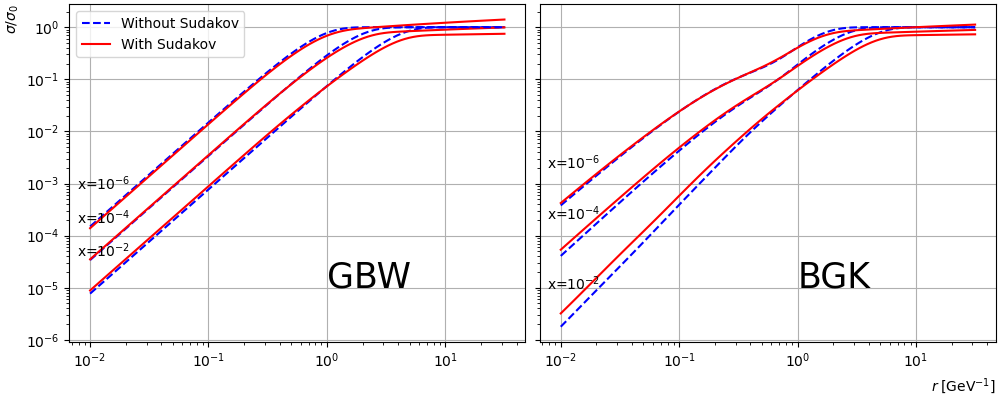
\includegraphics{./Plots/dipole-GBW.png}
}
%\resizebox{0.5\textwidth}{!}{
%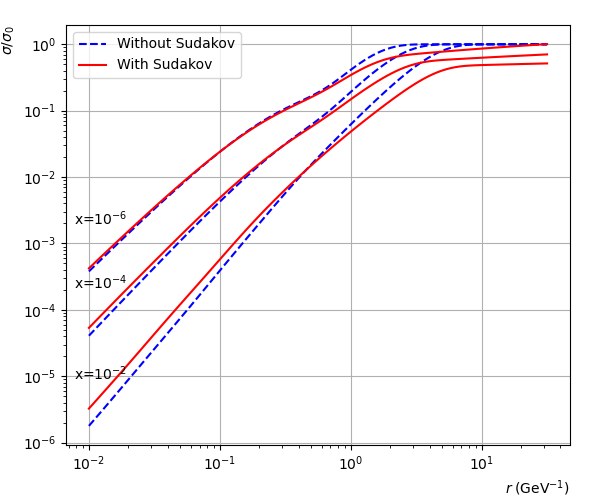
\includegraphics{./Plots/dipole-BGK.png}
%}
\caption{The dipole cross-section $\sigma_{\mathrm{dp}}$ at $Q^2=100\;\mathrm{GeV^2}$, and $x=10^{-2},10^{-4}, 10^{-6}$ (from bottom to top).\\Left: GBW, Right: BGK}
%\label{dipole-bgk}
\label{dipole}
\end{figure}

The effect of the Sudakov factor in the structure function, $F_2$, is shown in the Fig.~\ref{F2}. The changes are less obvious compared to the dipole cross-section, which is because the large-$r$ region, where the dipole cross-section was affected the most, is largely suppressed by the photon wave function.  Nonetheless, for both models the effect of the modification makes the increase of $F_2$ with $1/x$ milder (i.e., lowering the effective slope $\lambda_\mathrm{eff}=-\frac{\partial \log F_2}{\log x}$. cf. Fig~\ref{slope}), %({\color{red} easier to see in the plot of the slope})
and to lower $F_2$ in the large and small-$Q^2$ region (This can also be seen in Figs.~\ref{fig:gridGBW} and \ref{fig:gridBGK}). 
The unintegrated gluon distributions obtained from the models are shown in Figs.~\ref{fig:gluon} and \ref{fig:gluon-x}. As discussed in the previous section, the unintegrated gluon distributions from the modified models do not vanish in the limit $k^2\rightarrow0$. Both models show large change in the distribution, and the distribution appears to be smeared out both over $k^2$ and $x$, particularly, towards the low-$k^2$ and low-$x$ regions. As a result of the smearing effect, one can see in the BGK model, that the region where the gluon density was negative is lifted up.   
Although the shape of the distribution changes, the position of the peak remains at about the same place, implying little modification to the saturation scale (cf. Fig.~\ref{fig:critical}). 


\begin{figure}[p]
\resizebox{0.5\textwidth}{!}{
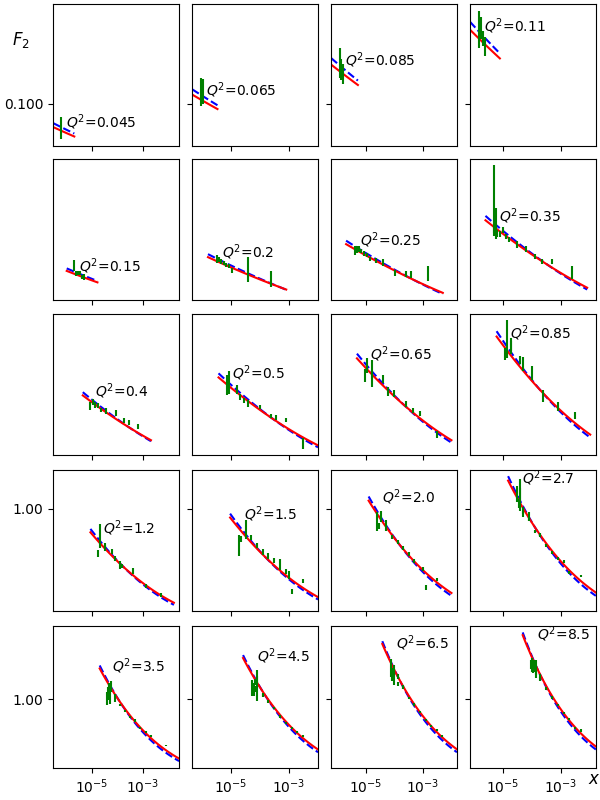
\includegraphics{./Plots/F2-data-GBW1.png}
}
\resizebox{0.5\textwidth}{!}{
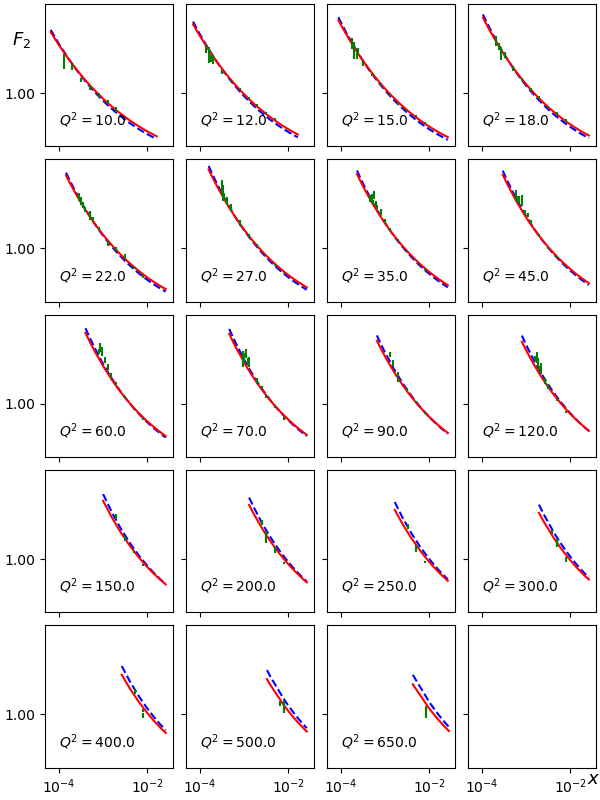
\includegraphics{./Plots/F2-data-GBW2.png}
}
\resizebox{\textwidth}{!}{
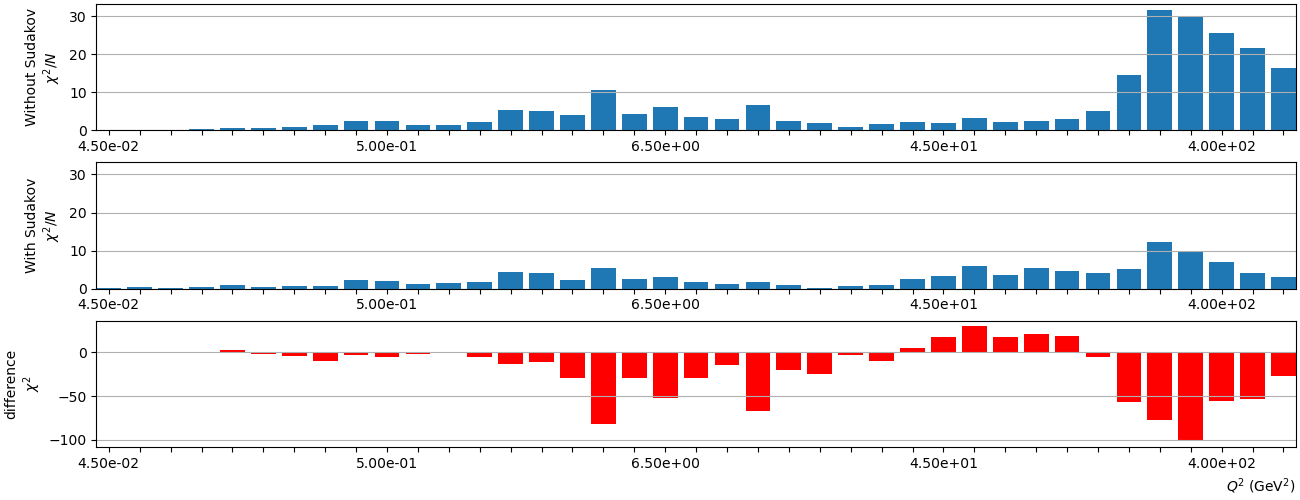
\includegraphics{./Plots/F2-data-GBWhist.png}
}
\caption{Top: $F_2$. GBW (Dashed blue) and GBWS (Solid red) and HERA data (Error bars), with fixed values of $Q^2$. Bottom: $\chi^2/\text{(no. of points)}$, and the difference $\chi^2_{\mathrm{GBWS}}-\chi^2_{\mathrm{GBW}}$ between GBW and GBWS models. Significant improvement at large $Q^2$ is clearly visible.}
\label{fig:gridGBW}
\end{figure}

\begin{figure}[p]
\resizebox{0.5\textwidth}{!}{
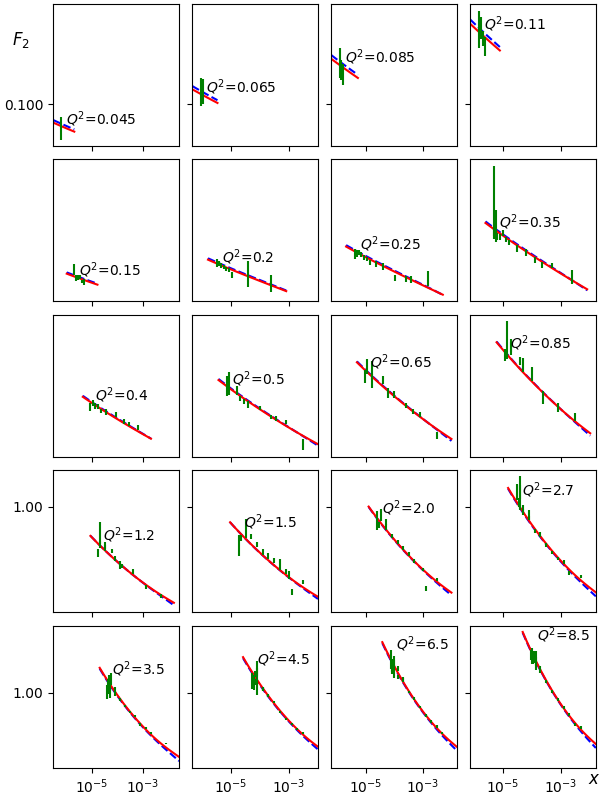
\includegraphics{./Plots/F2-data-BGK1.png}
}
\resizebox{0.5\textwidth}{!}{
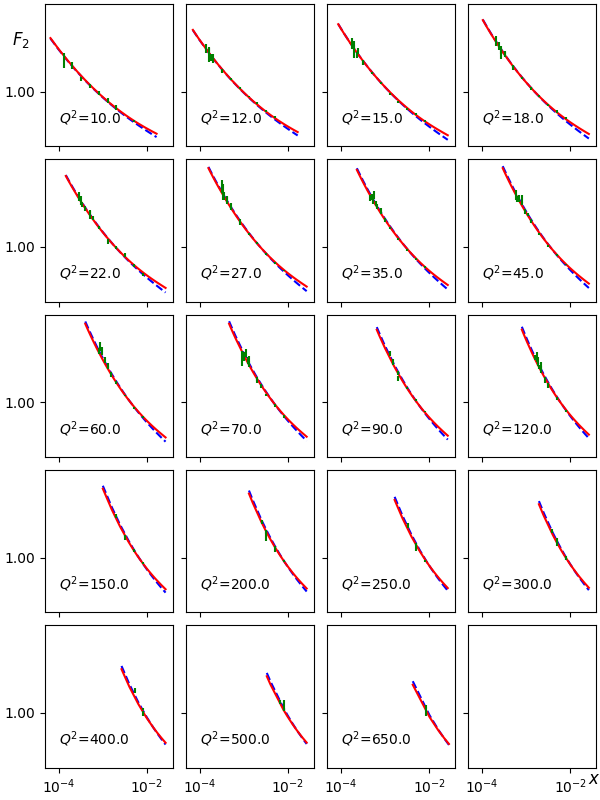
\includegraphics{./Plots/F2-data-BGK2.png}
}
\resizebox{\textwidth}{!}{
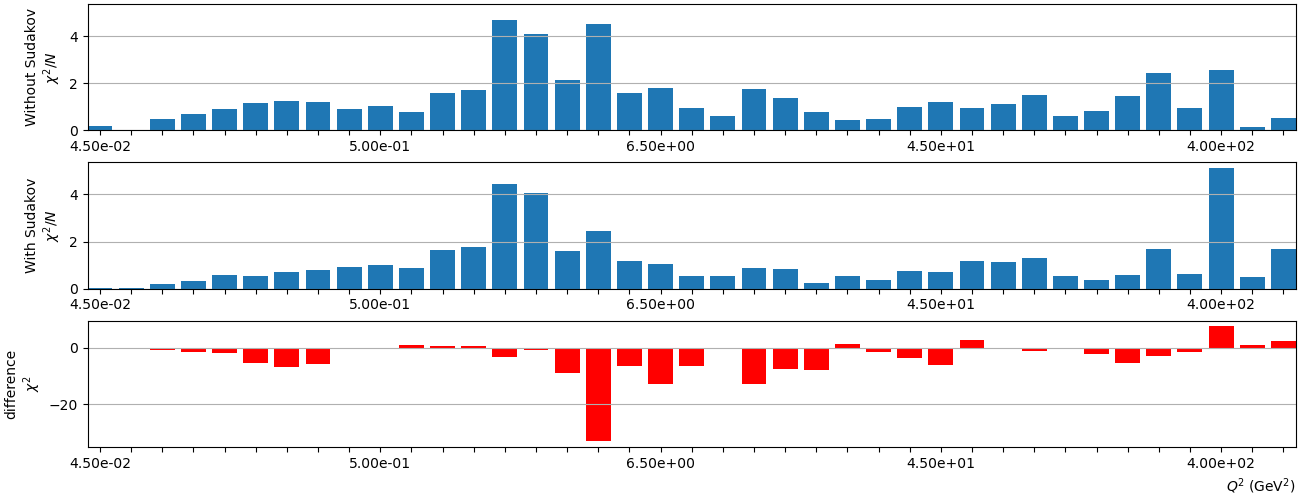
\includegraphics{./Plots/F2-data-BGKhist.png}
}
\caption{
Top: $F_2$. BGK (Dashed blue) and BGKS (Solid red) and HERA data (Error bars), with fixed values of $Q^2$. Bottom: $\chi^2/\text{(no. of points)}$, and the difference $\chi^2_{\mathrm{BGKS}}-\chi^2_{\mathrm{BGK}}$ between BGK and BGKS models.}
\label{fig:gridBGK}
\end{figure}

\begin{figure}[H]
\resizebox{\textwidth}{!}{
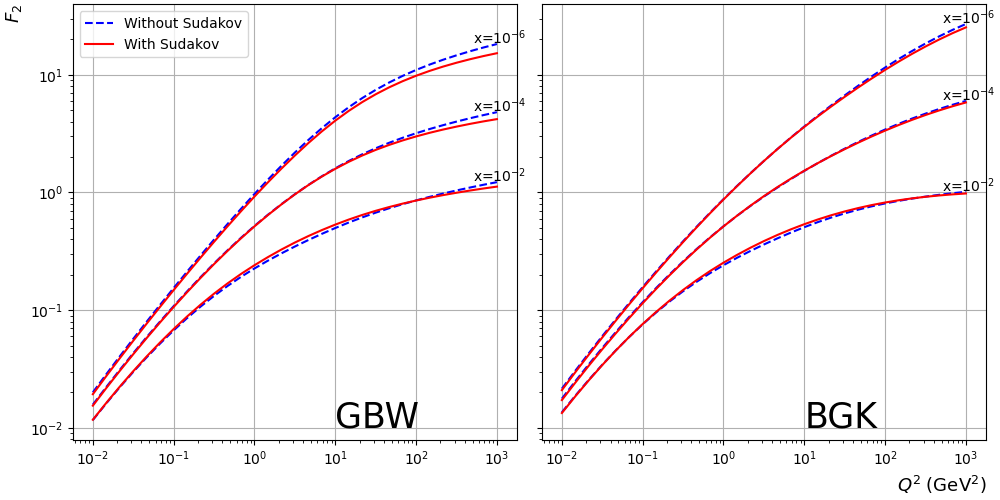
\includegraphics{./Plots/F2-GBW.png}
}
%\resizebox{0.5\textwidth}{!}{
%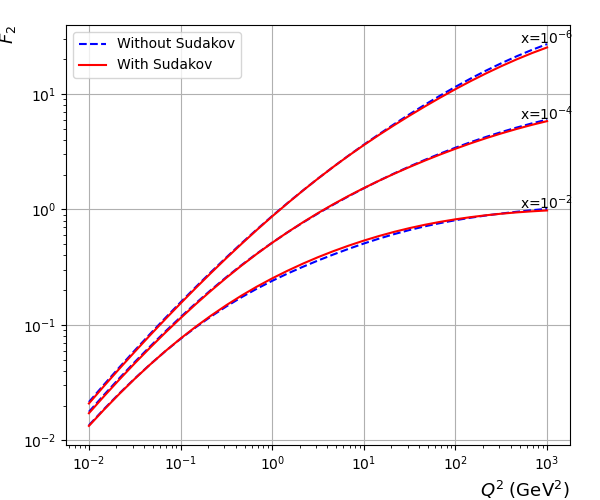
\includegraphics{./Plots/F2-BGK.png}
%}
\caption{The structure function $F_2$ , and $x=10^{-2}, 10^{-4}, 10^{-6}$ (from bottom to top).\\Left: GBW, Right: BGK}
\label{F2}
\end{figure}
\begin{figure}[H]
\resizebox{\textwidth}{!}{
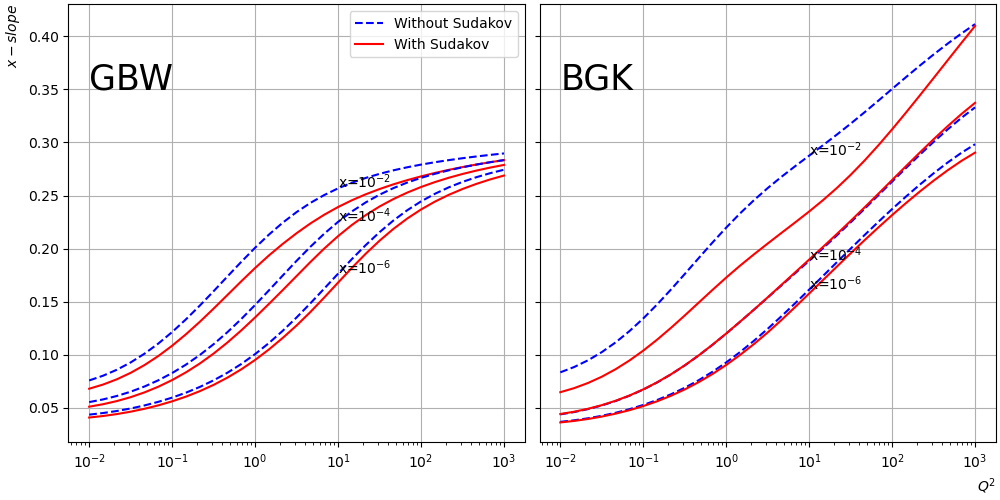
\includegraphics{./Plots/slope-GBW.png}
}
\caption{The $x$-slope of $F_2$,  $\lambda_\mathrm{eff}=-\frac{\partial \log F_2}{\log x}$,  and $x=10^{-2},10^{-4}, 10^{-6}$ (from bottom to top). The slope is generally lowered, and this can be seen also in Figs.~\ref{fig:gridGBW} and \ref{fig:gridBGK}\\Left: GBW, Right: BGK}
\label{slope}
\end{figure}


\begin{figure}[H]
\resizebox{\textwidth}{!}{
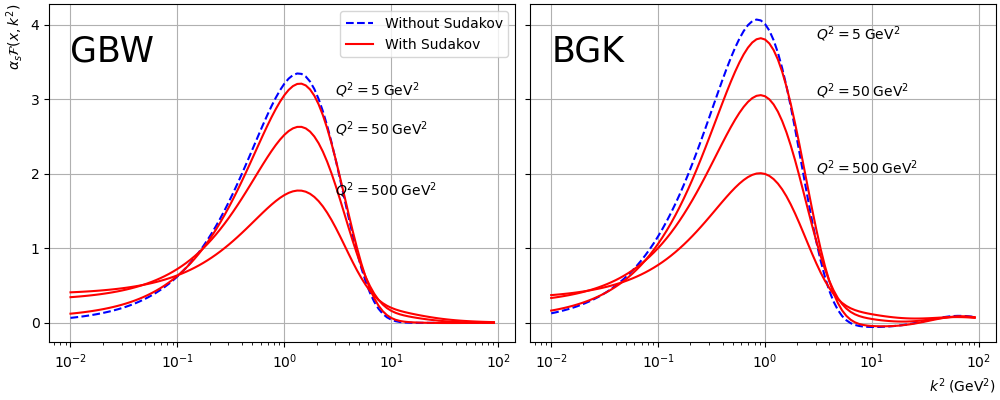
\includegraphics{./Plots/gluon-GBW.png}
}
%\resizebox{0.5\textwidth}{!}{
%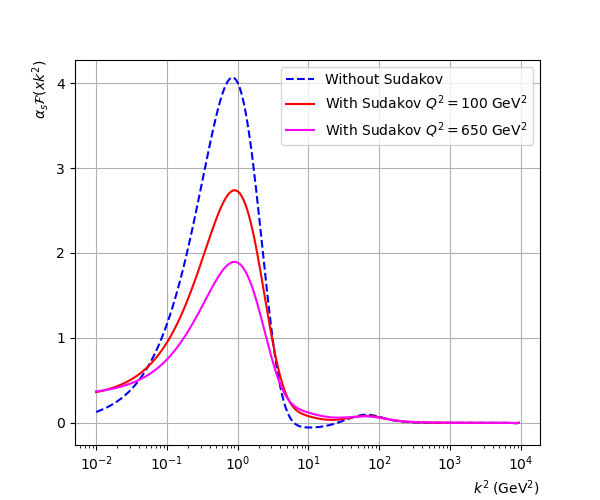
\includegraphics{./Plots/gluon-BGK.png}
%}
\caption{$\alpha_s\mathcal{F}(x,k^2)$ plotted for $x=10^{-4}$ and $Q^2=5, 50 , 500\; \mathrm{GeV^2}$ (from top to bottom). Notice the broadening effect of the Sudakov factor, particularly towards the small value of $k^2$.\\Left: GBW, Right: BGK}
\label{fig:gluon}
\end{figure}
\begin{figure}[H]
\resizebox{\textwidth}{!}{
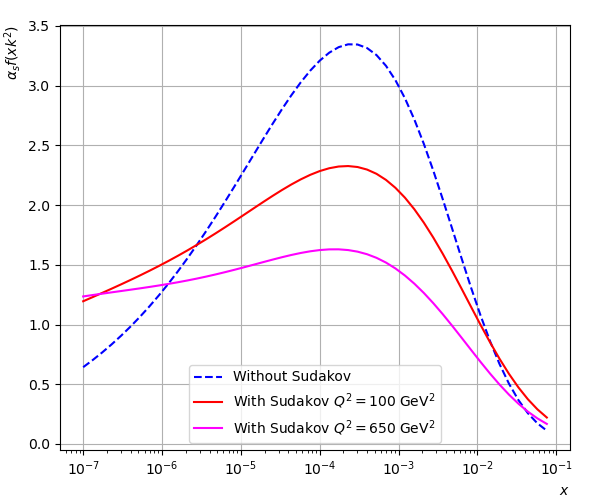
\includegraphics{./Plots/gluon-x-GBW.png}
}
%\resizebox{0.5\textwidth}{!}{
%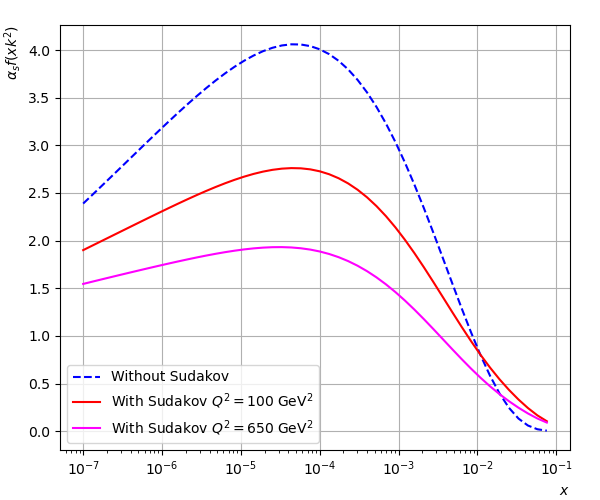
\includegraphics{./Plots/gluon-x-BGK.png}
%}
\caption{$\alpha_s\mathcal{F}(x,k^2)$ plotted for $k^2=1\;\mathrm{GeV^2}$ and $Q^2=5, 50 , 500\; \mathrm{GeV^2}$ (from top to bottom). Notice the broadening effect of the Sudakov factor, particularly towards the small value of $x$.\\Left: GBW, Right: BGK}
\label{fig:gluon-x}
\end{figure}

As one can see in Fig.~\ref{dipole}, the dipole cross-section starts to bend somewhat earlier due to the Sudakov factor. For the small value of $Q^2$ near the expected saturation scale, the effect of the Sudakov factor is relatively small, yet this causes the saturation to take effect earlier and at the same time, the transition becomes slower. This means that the critical line becomes less clear as transition becomes milder over a wider range. % As discussed earlier, the definition of the saturation scale in terms of the dipole cross-section becomes less clear.
Comparisons of $x$-dependent saturation scale are presented in Fig.~\ref{fig:critical}. While the change in the GBW model  are only in the slope, the saturation scale of  BGK model becomes higher for the whole range of $x$, implying the saturation effect to show at slightly higher scale than expected from the original models.
{\color{blue}Finally, we present the longitudinal sturucture function $F_L$ in Fig.~\ref{fig:FL} with H1 data \cite{FL}. Both the GBW and BGK models show similar effects from the Sudakov factor. The main effects are in the large-$Q^2$ region, and for both the models, $F_L$ is higher when the Sudakov factor is present. }
%{\color{pink}Comparisons of $x$-dependent saturation scale are presented in Fig.~\ref{fig:critical}. While the change in GBW model from the definition Eq.~(\ref{eq:peak}) are only in the slope, the saturation scale of the BGK model and that of the GBW model from the definition Eq.~(\ref{eq:curvature}) becomes higher, implying the saturation effect to show at slightly higher scale than expected from the original models.} %{\color{red}$Q^2$ dependence of the saturation scale? what to show? ``peak'' version has no noticeable dependence. } 

\begin{figure}[H]
\resizebox{\textwidth}{!}{
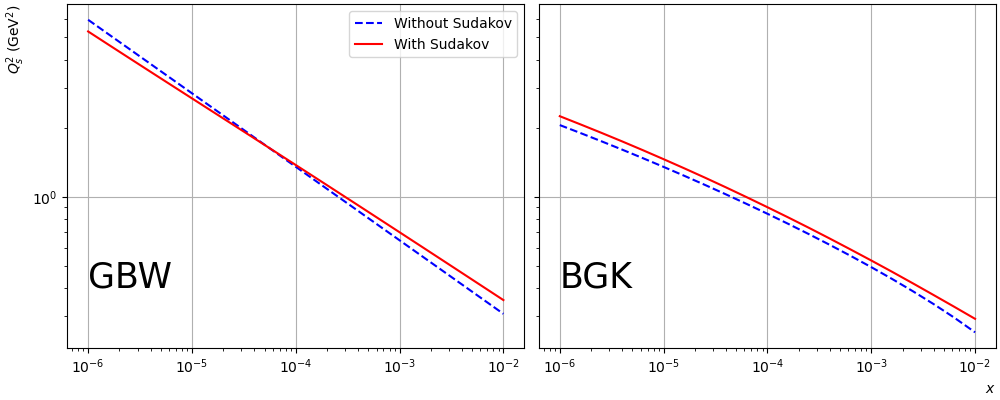
\includegraphics{./Plots/critical-GBW.png}
}
%\resizebox{0.5\textwidth}{!}{
%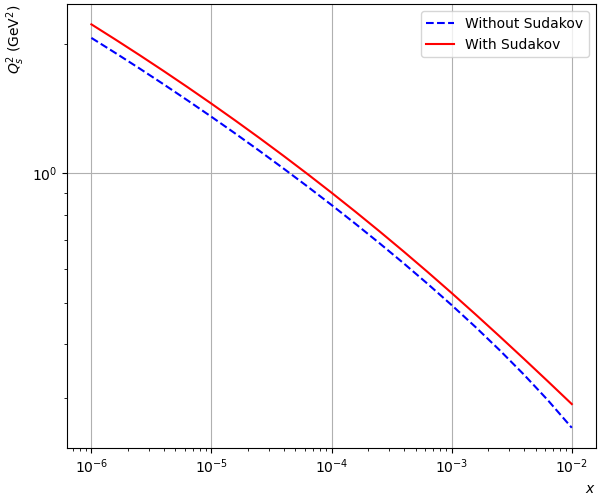
\includegraphics{./Plots/critical-BGK.png}
%}
\caption{Saturation scale $Q_s^2(x)$.
%\caption{Saturation scale $Q_S^2(x)$  obtained from two different criteria:\\
%$\frac{\partial^2 \sigma }{\partial r^2}=0$ (Curvature) \& $\frac{\partial \alpha_s\mathcal{F}(x,k^2) }{\partial k}=0$ (Peak).\\ 
The line was plotted for $Q^2=100\;\mathrm{ GeV^2}$.\\Left: GBW, Right: BGK }
\label{fig:critical}
\end{figure}


\begin{figure}[H]
\resizebox{\textwidth}{!}{
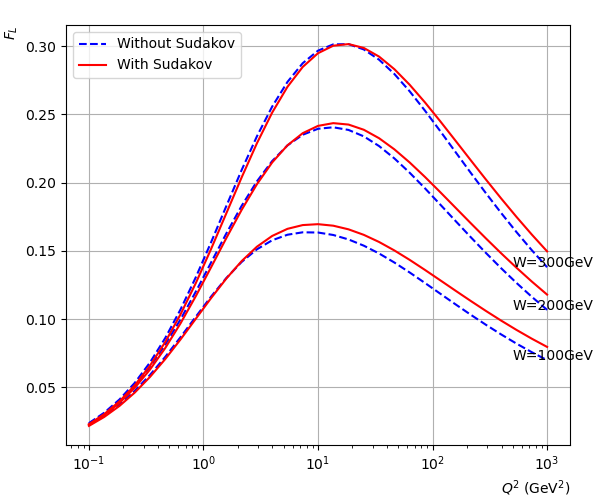
\includegraphics{./Plots/FL-GBW.png}
}
%\resizebox{0.5\textwidth}{!}{
%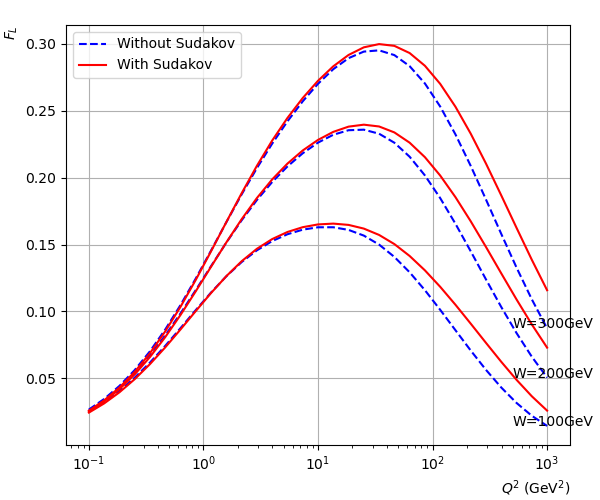
\includegraphics{./Plots/FL-BGK.png}
%}
\caption{The longitudinal structure function, $F_L$, at fixed $W=100, 200, 300$ GeV (from bottom to top).
The effects of the Sudakov factor is primarily in the large-$Q^2$ region, lifting up the line for both the GBW and BGK models.
The data are from Ref.~\cite{FL}.\\
Left: GBW, Right: BGK}
\label{fig:FL}
\end{figure}

\section{Summary}
In this paper we have presented the effects of the Sudakov form factor in the Golec-Biernat W\"ustfoff (GBW) model and the Bartels Golec-Biernat Kowalski (BGK) model. 
The leading order Sudakov factor was inserted in the model via modifying the unintegrated gluon density. This renders the dipole cross-section $Q^2$-dependent.
The results of fittings with the HERA data in the range $0.045\mathrm{GeV} \leq Q^2 \leq 650\mathrm{GeV}$ and $x\leq 10^{-2}$ have shown improvements in both models and most importantly, the BGK model exhibits good behaviour over a wide range of $Q^2$.  In terms of the dipole cross-section, the Sudakov factor modifies it in the region $1/r\lesssim Q$ by lowering initially and allowing logarithmic rise in the large-$r$ region.  This, in the light of the saturation effect, means that saturation starts earlier and the transition to the saturation region becomes slower. The effect is stronger for a large value of $Q^2$ and disappears when $Q^2=0$. In other words, the photoproduction is unaffected by the Sudakov factor and the sole change comes from the change in the fit parameters. The present study was conducted for inclusive DIS, however diffractive DIS is {\color{blue}even} more sensitive to the large-$r$ region where the effect of the Sudakov factor is more prominent. Therefore, one may gain further insight on the effects by studying the diffractive processes,which we leave for future works.


%%%%%%%%%%%%%%%%%%%%%%%%%%%%%%%%%%%%%%%%%%%%%%%%%%%%%%%%%%%%%%%%%%%%%%%%%%%
%\newpage
\printbibliography
%%%%%%%%%%%%%%%%%%%%%%%%%%%%%%%
\appendix
\section{Miscellaneous plots}





\begin{figure}[H]
\resizebox{\textwidth}{!}{
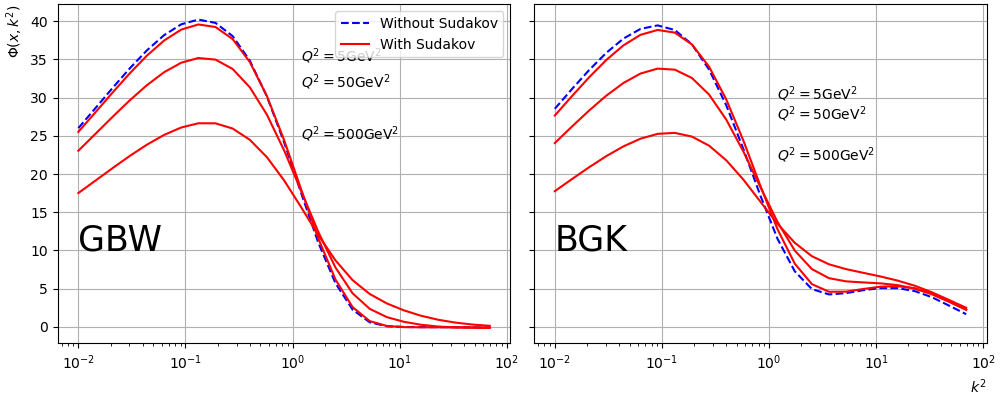
\includegraphics{./Plots/ww-gluon-GBW.png}
}
%\resizebox{0.5\textwidth}{!}{
%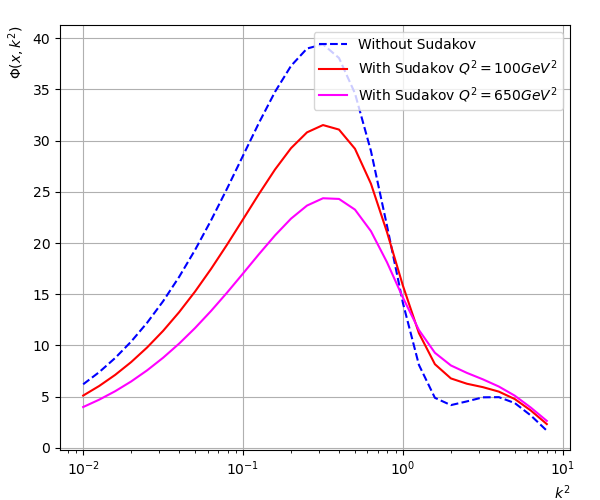
\includegraphics{./Plots/ww-gluon-BGK.png}
%}
\caption{Weizs\"acke-Williams gluon distrubution $\phi=k\int \frac{d^2r}{r^2} e^{-i r\cdot k} \sigma_{\mathrm{dp}}(x,r,Q^2)$.\\Left: GBW, Right: BGK
}
%\label{fig:gluon}
\end{figure}

\begin{figure}[H]
\resizebox{\textwidth}{!}{
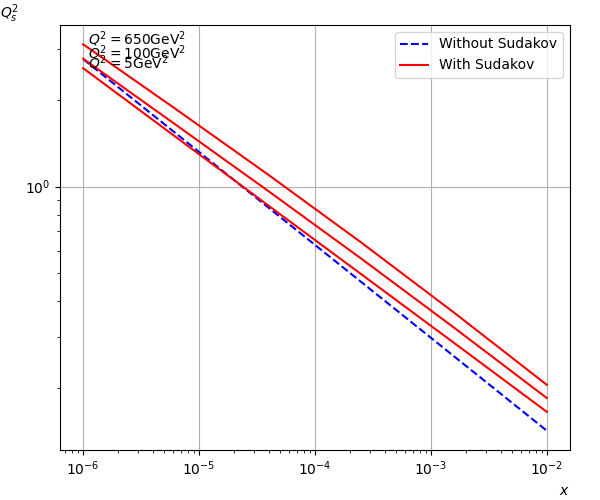
\includegraphics{./Plots/ww-critical-GBW.png}
}
%\resizebox{0.5\textwidth}{!}{
%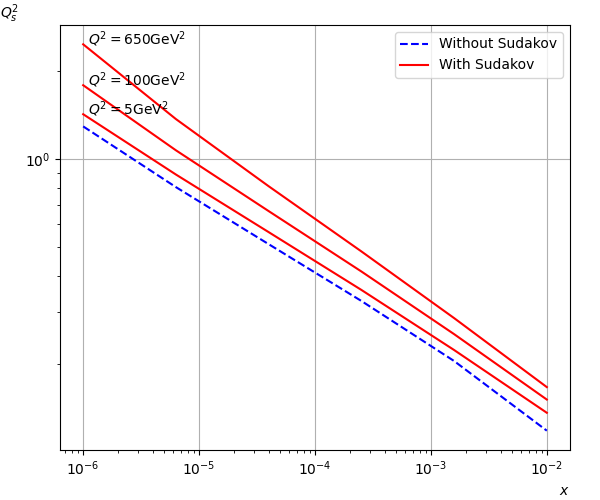
\includegraphics{./Plots/ww-critical-BGK.png}
%}
\caption{Saturation scale $Q_s^2(x)$  obtained from the Weiz\"acker-Williams gluon distribution.
The crieria is analogous to Eq.~(\ref{eq:peak}) for $\phi=k\int \frac{d^2r}{r^2} e^{-i r\cdot k} \sigma_{\mathrm{dp}}(x,r,Q^2)$ but with an extra factor 2 as in the original GBW saturation scale.  i.e., $Q_s=2 k_s$.\\Left: GBW, Right: BGK }
%\label{fig:critical}
\end{figure}


\end{document}